\begin{figure}[!ht]
	\centering
	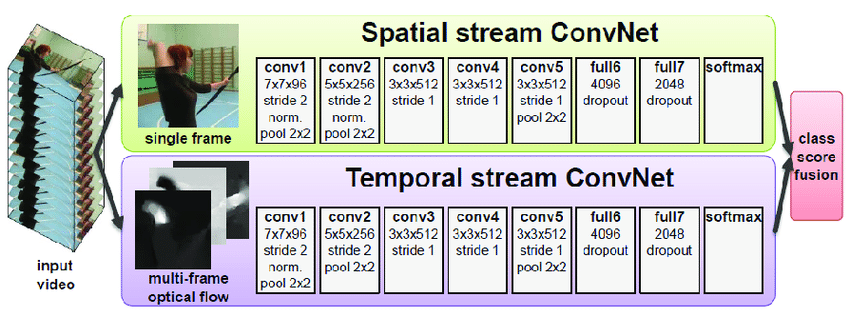
\includegraphics[width=1\textwidth]{chapter2/images/2steamCNN.png}
		\caption{แสดงโครงสร้างการทำงานของ two stream}
    	\label{fig:/2steamCNN}
\end{figure}

Two-Steam CNN \footnote{2steamCNN,https://papers.nips.cc/paper/5353-two-stream-convolutional-networks-for-action-recognition-in-videos.pdf} 
เป็นวิธีการหนึ่งในการทำ video classification โดยจะแบ่งออกเป็นสองกระบวนการทำไปพร้อมกัน คือ 
กระบวนการแรกนำรูปภาพเดี่ยวๆ มาใช้ซึ่งจะทำให้ได้ข้อมูลจากรูปภาพคือ ฉากและวัตถุต่างๆ และ 
กระบวนการที่สองนำลำดับของรูปภาพมาเพื่อดูการเคลื่อนไหวของวัตถุ 
และสุดท้ายจะนำข้อมูลที่ได้จากทั้งสองกระบวนการมารวมกันโดยใช้การ 
averaging หรือนำไปผ่าน linear SVM 
